\section{Exercise 1: Zenith Troposphere Delay estimation}


Questions:
\begin{enumerate}
\item What is the level of discrepancy between the estimated ZTD and the accurate IGS determination?
\item What is the variation of ZTD in 24 hours due to the wet content?
\item What is the proportion of wet component compared with the dry (or hydrostatic) component?
\end{enumerate}


First of all, to make the labs, a Debian SO has been used. Introducing the following command $lsb_release -a$ we obtain the following output:\\


\begin{figure}[h]
    \centering
    \begin{minted}[fontsize=\footnotesize, bgcolor=bg, breaklines, tabsize=2, frame=lines, framesep=2mm]{console}
        marc@debian:~$ lsb_release -a
        No LSB modules are available.
        Distributor ID: Debian
        Description:    Debian GNU/Linux 11 (bullseye)
        Release:        11
        Codename:       bullseye
    \end{minted}
    \caption{Random noise signal and its representation using Matplotlib. The data has been extracted and plotted using Python.
    }
    \label{fig:Ejemplo de código de bash}
\end{figure}


\begin{figure}[H]
        \centering
        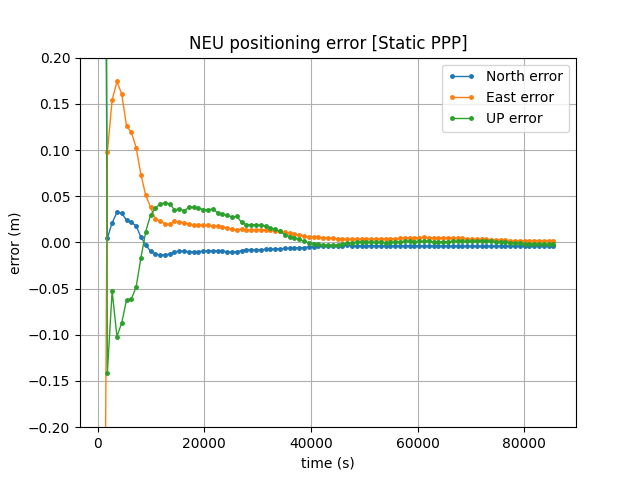
\includegraphics[scale=0.52]{sources/Figures/FIG_2/TUT2_Ex1a.png}
        \caption{}
        \label{fig:}
\end{figure}



\begin{figure}[H]
        \centering
        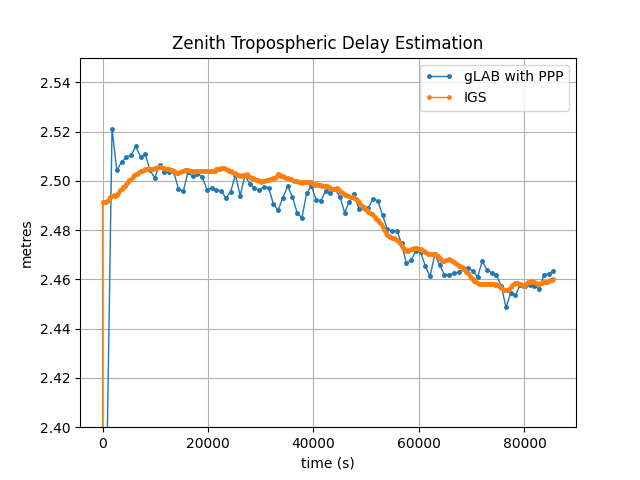
\includegraphics[scale=0.52]{sources/Figures/FIG_2/TUT2_Ex1b.png}
        \caption{}
        \label{fig:}
\end{figure}

\begin{figure}[H]
    \centering
    \begin{subfigure}{0.45\textwidth}
        \centering
        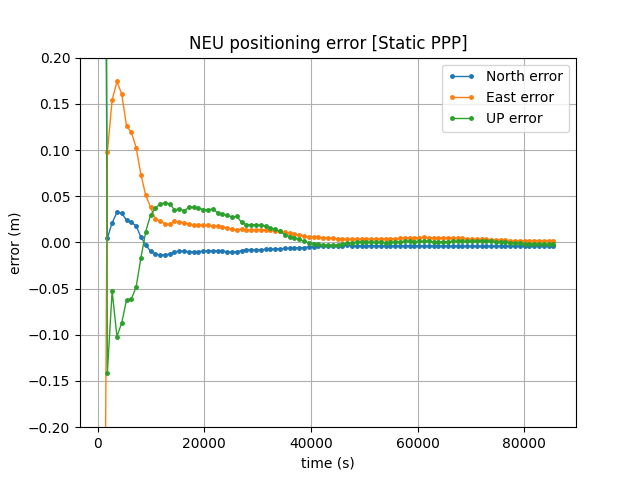
\includegraphics[scale=0.52]{sources/Figures/FIG_2/TUT2_Ex1a.png}
        \caption{}
        \label{fig:subfig1}
    \end{subfigure}
    \hfill
    \begin{subfigure}{0.45\textwidth}
        \centering
        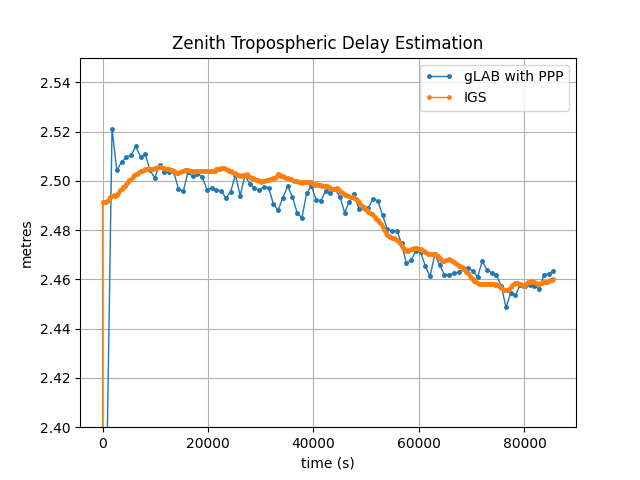
\includegraphics[scale=0.52]{sources/Figures/FIG_2/TUT2_Ex1b.png}
        \caption{}
        \label{fig:subfig2}
    \end{subfigure}
    \caption{}
    \label{fig:dos-figuras-juntas}
\end{figure}